\documentclass[t,usenames,dvipsnames]{beamer}
\usetheme{Copenhagen}
\setbeamertemplate{headline}{} % remove toc from headers
\beamertemplatenavigationsymbolsempty

\usepackage{amsmath, xcolor, tikz, pgfplots, bm}

\pgfplotsset{compat = 1.16}
\usetikzlibrary{arrows.meta, calc, decorations.pathreplacing}
\pgfplotsset{every axis/.append style = {axis lines = middle}}
\pgfplotsset{every tick label/.append style={font=\scriptsize}}
\everymath{\displaystyle}

\title{Dividing Polynomials}
\author{}
\date{}

\AtBeginSection[]
{
  \begin{frame}
    \frametitle{Objectives}
    \tableofcontents[currentsection]
  \end{frame}
}

\begin{document}

\begin{frame}
    \maketitle
\end{frame}

\section{Divide polynomials without a remainder}

\begin{frame}{Division Basics}
In the expression $a \div b = c$, $a$ is the \alert{dividend}, $b$ is the \alert{divisor}, and $c$ is the \alert{quotient}.   \newline\\

When dividing polynomials, it will help to write your terms in standard form (descending powers). You may also need to fill in any missing terms using 0 as a coefficient. \newline\\

Before we get to division, let's review an organizational technique for multiplying polynomials.
\end{frame}

\begin{frame}{Multiplication Example}
To find the product of $(x-2)(x^2+6x+7)$, we can use the following method:   
\begin{center}
    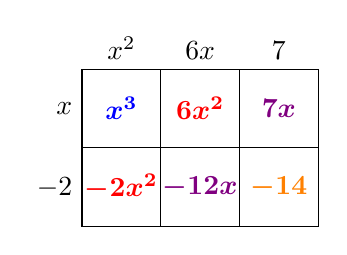
\begin{tikzpicture}
    \draw (0,0) grid (3,2);
    \node at (0,1.5) [left] {$x$};
    \node at (0,0.5) [left] {$-2$};
    \node at (0.5,2) [above] {$x^2$};
    \node at (1.5,2) [above] {$6x$};
    \node at (2.5,2) [above] {7};
    \onslide<2->{\node at (0.5,1.5) {\color{blue}$\bm{x^3}$};}
    \onslide<4->{\node at (1.5,1.5) {\color{red}$\bm{6x^2}$};}
    \onslide<3->{\node at (0.5,0.5) {\color{red}$\bm{-2x^2}$};}
    \onslide<5->{\node at (1.5,0.5) {\color{violet}$\bm{-12x}$};}
    \onslide<6->{\node at (2.5,1.5) {\color{violet}$\bm{7x}$};}
    \onslide<7->{\node at (2.5,0.5) {\color{orange}$\bm{-14}$};}
    \end{tikzpicture}
\end{center}
\onslide<8->{
When we combine all of terms inside the box, we get the product, $x^3 + 4x^2 - 5x - 14$.}
\end{frame}

\begin{frame}{Division}
We can reverse the process using division to find the quotient
\[
(x^3 + 4x^2 - 5x - 14) \div (x - 2)
\]
\begin{center}
    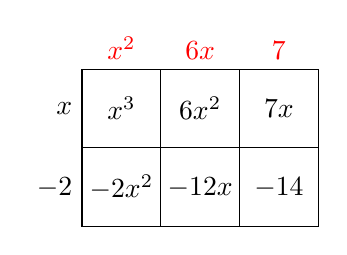
\begin{tikzpicture}
    \draw (0,0) grid (3,2);
    \node at (0,1.5) [left] {$x$};
    \node at (0,0.5) [left] {$-2$};
    \node at (0.5,1.5) {$x^3$};
    \onslide<2->{\node at (0.5,2) [above] {\color{red}$x^2$};}
    \onslide<3->{\node at (0.5,0.5) {$-2x^2$};}
    \onslide<4->{\node at (1.5,1.5) {$6x^2$};}
    \onslide<5->{\node at (1.5,2) [above] {\color{red}$6x$};}
    \onslide<6->{\node at (1.5,0.5) {$-12x$};}
    \onslide<8->{\node at (2.5,2) [above] {\color{red}$7$};}
    \onslide<7->{\node at (2.5,1.5) {$7x$};}
    \onslide<9->{\node at (2.5,0.5) {$-14$};}
\end{tikzpicture}
\end{center}
\onslide<10->{\[x^2 + 6x + 7\]}
\end{frame}

\begin{frame}{Example 1}
Divide $(x^3+8) \div (x+2)$
\onslide<2->{\[(x^3 + 0x^2 + 0x + 8) \div (x+2)\]}
\begin{center}
\onslide<3->{
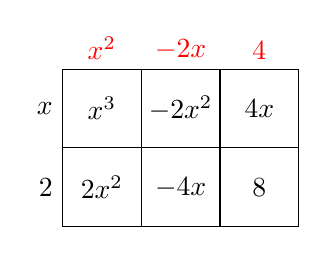
\begin{tikzpicture}
\draw (0,0) grid (3,2);
\node at (0,1.5) [left] {$x$};
\node at (0,0.5) [left] {2};
\onslide<4->{\node at (0.5,1.5) {$x^3$};}
\onslide<5->{\node at (0.5,2) [above] {\color{red}$x^2$};}
\onslide<6->{\node at (0.5,0.5) {$2x^2$};}
\onslide<7->{\node at (1.5,1.5) {$-2x^2$};}
\onslide<8->{\node at (1.5,2) [above] {\color{red}$-2x$};}
\onslide<9->{\node at (1.5,0.5) {$-4x$};}
\onslide<10->{\node at (2.5,1.5) {$4x$};}
\onslide<11->{\node at (2.5,2) [above] {\color{red}4};}
\onslide<12->{\node at (2.5,0.5) {8};}
\end{tikzpicture}} \vspace{8pt}
\end{center}
\onslide<13->{\[\color{red}{x^2 - 2x + 4}\]}
\end{frame}


\section{Divide polynomials with a remainder}

\begin{frame}{Dividing Polynomials With a Remainder}
In the previous examples, everything ``balanced out" from within the grid. \newline\\

In other words, after combining like terms, all terms in the dividend were accounted for.    \newline\\  \pause

In the next group of examples, we will need to figure out what to add to our quotient to ``balance out the problem."  \newline\\  

We will write our answers in the form 
\[
\text{quotient} + \frac{\text{remainder}}{\text{divisor}}
\]
\end{frame}

\begin{frame}{Example 2}
Divide each.    \newline\\
(a) \quad $(5x^3 - 2x^2 + 1) \div (x-3)$
\onslide<2->{\[(5x^3 - 2x^2 + 0x + 1) \div (x-3) \]}
\onslide<3->{
\begin{center}
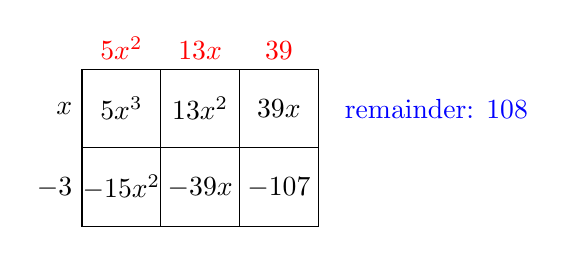
\begin{tikzpicture}
\draw (0,0) grid (3,2);
\node at (0,1.5) [left] {$x$};
\node at (0,0.5) [left] {$-3$};
\onslide<4->{\node at (0.5,1.5) {$5x^3$};}
\onslide<5->{\node at (0.5,2) [above] {\color{red}$5x^2$};}
\onslide<6->{\node at (0.5,0.5) {$-15x^2$};}
\onslide<7->{\node at (1.5,1.5) {$13x^2$};}
\onslide<8->{\node at (1.5,2) [above] {$\color{red}13x$};}
\onslide<9->{\node at (1.5,0.5) {$-39x$};}
\onslide<10->{\node at (2.5,1.5) {$39x$};}
\onslide<11->{\node at (2.5,2) [above] {$\color{red}39$};}
\onslide<12->{\node at (2.5,0.5) {$-107$};}
\onslide<13->{\node at (4.5,1.5) {$\color{blue}\text{remainder: }108$};}
\end{tikzpicture}
\end{center}}
\end{frame}


\begin{frame}{Example 2}
(a) \quad $(5x^3 - 2x^2 + 1) \div (x-3)$

\[ 5x^2 + 13x + 39 \text{ remainder: } 108  \]  \vspace{12pt}   \pause

\[ 5x^2 + 13x + 39 + \frac{108}{x-3} \]
\end{frame}

\begin{frame}{Example 2}
(b) \quad $(4-8x-12x^2) \div (2x-3)$
\onslide<2->{\[(-12x^2 - 8x + 4) \div (2x-3)\]}
\onslide<3->{
\begin{center}
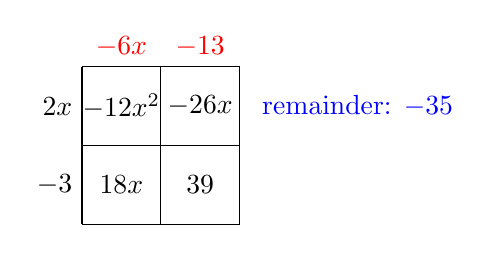
\begin{tikzpicture}
\draw (0,0) grid (2,2);
\node at (0,1.5) [left] {$2x$};
\node at (0,0.5) [left] {$-3$};
\onslide<4->{\node at (0.5,1.5) {$-12x^2$};}
\onslide<5->{\node at (0.5,2) [above] {\color{red}$-6x$};}
\onslide<6->{\node at (0.5,0.5) {$18x$};}
\onslide<7->{\node at (1.5,1.5) {$-26x$};}
\onslide<8->{\node at (1.5,2) [above] {$\color{red}-13$};}
\onslide<9->{\node at (1.5,0.5) {$39$};}
\onslide<10->{\node at (3.5,1.5) {\color{blue}\text{remainder: }$-35$};}
\end{tikzpicture}
\end{center}}
\end{frame}

\begin{frame}{Example 2}
(b) \quad $(4-8x-12x^2) \div (2x-3)$
\[-6x - 13 \text{remainder } -35 \] \pause
\[ -6x - 13 - \frac{35}{2x-3}\]
\end{frame}

\begin{frame}{Example 2}
(c) \quad   $(3x^3 + 4x^2 + x + 7) \div (x^2 + 1)$  
\onslide<2->{\[(3x^3 + 4x^2 + x + 7) \div (x^2 + 0x + 1)\]}
\onslide<3->{
\begin{center}
    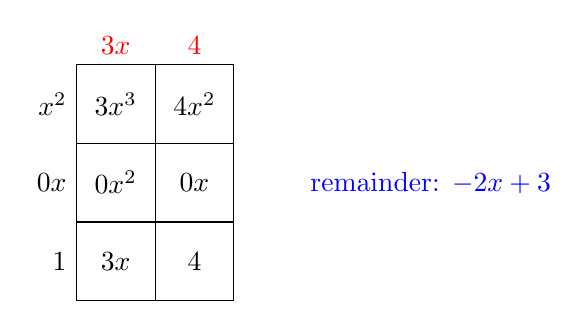
\begin{tikzpicture}
    \draw (0,0) grid (2,3);
    \node at (0,2.5) [left] {$x^2$};
    \node at (0,1.5) [left] {$0x$};
    \node at (0,0.5) [left] {$1$};
    \node at (0.5,2.5) {$3x^3$};
    \onslide<7->{\node at (1.5,2.5) {$4x^2$};}
    \onslide<5->{\node at (0.5,1.5) {$0x^2$};}
    \onslide<9->{\node at (1.5,1.5) {$0x$};}
    \onslide<6->{\node at (0.5,0.5) {$3x$};}
    \onslide<10->{\node at (1.5,0.5) {4};}
    \onslide<4->{\node at (0.5,3) [above] {\color{red}$3x$};}
    \onslide<8->{\node at (1.5,3) [above] {\color{red}$4$};}
    \onslide<11->{\node at (4.5,1.5) {\color{blue}\text{remainder: }$-2x+3$};}
\end{tikzpicture}
\end{center}}
\end{frame}

\begin{frame}{Example 2}
(c) \quad   $(3x^3 + 4x^2 + x + 7) \div (x^2 + 1)$ 
\[ 3x + 4 \text{remainder } -2x+3 \]
\onslide<2->{\[3x + 4 + \frac{-2x+3}{x^2+1}\]}
\end{frame}

\section{Use the Remainder Theorem and Factor Theorem}

\begin{frame}{The Remainder Theorem}
There is a quicker way to determine if some polynomial division problems result in a remainder. \newline\\

\begin{center}
    \textbf{The Remainder Theorem}  \newline\\
    If $p$ is a polynomial of degree at least 1, and $c$ is a real number, then when $p(x)$ is divided by $x-c$, the remainder is $p(c)$.
\end{center}
\end{frame}

\begin{frame}{Example 3}
What is the remainder when $2x^3 - 5x + 3$ is divided by $x+2$? 
\begin{align*}
   \onslide<2->{p(-2) &= 2(-2)^3 - 5(-2) + 3} \\
   \onslide<3->{p(-2) &= -3}    \\
\end{align*}
\onslide<4->{The remainder is $-3$}
\end{frame}

\begin{frame}{The Factor Theorem}
    \alert{The Factor Theorem} states that if $p$ is a nonzero polynomial, then the real number $c$ is a zero of $p$ if $(x-c)$ is a factor of $p(x)$. \newline\\   \pause
    
    In other words, $p(c) = 0$.
\end{frame}

\begin{frame}{Example 4}
Use the fact that $x = 1$ is a zero of $p(x) = 2x^3 - 5x + 3$ to factor $p(x)$ and find all of the real zeros of $p$.   \newline\\  
\onslide<2->{$(2x^3 + 0x^2 - 5x + 3) \div (x - 1)$ will have a remainder of 0.}   \newline\\
\begin{center}
\onslide<3->{
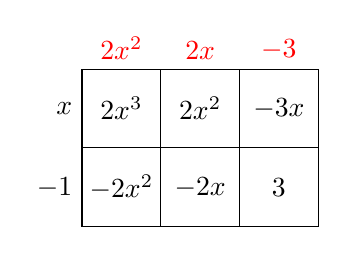
\begin{tikzpicture}
    \draw (0,0) grid (3,2);
    \node at (0,1.5) [left] {$x$};
    \node at (0,0.5) [left] {$-1$};
    \node at (0.5,1.5) {$2x^3$};
    \onslide<4->{\node at (0.5,2) [above] {\color{red}$2x^2$};}
    \onslide<5->{\node at (0.5,0.5) {$-2x^2$};}
    \onslide<6->{\node at (1.5,1.5) {$2x^2$};}
    \onslide<7->{\node at (1.5,2) [above] {\color{red}$2x$};}
    \onslide<8->{\node at (1.5,0.5) {$-2x$};}
    \onslide<9->{\node at (2.5,1.5) {$-3x$};}
    \onslide<10->{\node at (2.5,2) [above] {\color{red}$-3$};}
    \onslide<11->{\node at (2.5,0.5) {$3$};}
\end{tikzpicture}}
\end{center}
\end{frame}

\begin{frame}{Example 4}
\[ 2x^2 + 2x - 3 = 0 \] \pause
using the Quadratic Formula, we get
\[ x = \frac{-1\pm \sqrt{7}}{2}  \]
\end{frame}

\end{document}


